\documentclass[11pt]{article}   	
% use "amsart" instead of "article" for AMSLaTeX format
\usepackage{fullpage}
\usepackage{geometry}                		% See geometry.pdf to learn the layout options. There are lots.
\geometry{letterpaper, margin=1in}                   		% ... or a4paper or a5paper or ...
%\geometry{landscape}                		% Activate for rotated page geometry
%\usepackage[parfill]{parskip}    		% Activate to begin paragraphs with an empty line rather than an indent
\usepackage{graphicx}				% Use pdf, png, jpg, or eps§ with pdflatex; use eps in DVI mode
								% TeX will automatically convert eps --> pdf in pdflatex		
\usepackage{amssymb}
\usepackage[boxed, linesnumbered]{algorithm2e}
%SetFonts

%SetFonts
\usepackage{subfigure}

\usepackage{epstopdf}

\usepackage{multicol}

\newtheorem{theorem}{Theorem}%[section]
\newtheorem{lemma}[theorem]{Lemma}
\newtheorem{claim}[theorem]{Claim}
\newtheorem{fact}[theorem]{Fact}
\newtheorem{definition}[theorem]{Definition}
\newtheorem{property}[theorem]{Property}

\newcommand{\sq}{\hbox{\rlap{$\sqcap$}$\sqcup$}}
\newcommand{\qed}{\hspace*{\fill}\sq}

\newenvironment{proof}{\noindent {\bf Proof.}\ }{\qed\par\vskip 4mm\par}
\newenvironment{proofof}[1]{\bigskip \noindent {\bf Proof of #1:}\quad }
{\qed\par\vskip 4mm\par}

\newcommand{\latpim} {\mathcal{L}_{pim}}
\newcommand{\latcpu} {\mathcal{L}_{cpu}}
\newcommand{\latllc} {\mathcal{L}_{llc}}
\newcommand{\latato} {\mathcal{L}_{atomic}}
\newcommand{\latmes} {\mathcal{L}_{message}}
\newcommand{\Sp}{\mathcal{S}_{p}}

\title{PIM-Managed Concurrent Data Structures}
\author{}
\date{}							% Activate to display a given date or no date

\begin{document}
\maketitle

\begin{abstract}
The process-in-memory (PIM) model has reemerged and drawn a lot of attention recently, 
as breakthroughs on 3D die-stacked technology make PIM architectures viable. 
In the PIM model, some lightweight computing units, called PIM cores, are directly attached to 
the main memory, making memory access by PIM cores much faster than by CPUs. 
Researchers have already shown significant performance improvements on applications, 
such as embarrassingly parallel, data-intensive algorithms and 
pointer-chasing traversals in sequential data structures, in PIM architectures. 

In this paper, we explore ways to design efficient concurrent data structures in the PIM model. 
The concurrent data structures we consider include linked-list and skip-list, 
as examples of pointer-chasing data structures, 
and FIFO queue, as an example of contended data structures.  
Designing and implementing concurrent data structures with the normal DRAM memory 
is known to be notoriously hard for non-experts. 
We show that in the PIM model, PIM-managed concurrent data structures can be much simpler. 
With the help of different optimizations like combining, partitioning and pipelining, 
our PIM-managed concurrent data structures can in theory be better than, or at least as good as, 
all other existing algorithms we are aware of, based on our performance model. 
Our preliminary experiments that indirectly compare our PIM-managed concurrent data structures 
with other algorithms also indicate that our algorithms are expected to outperform others. 
\end{abstract}
\newpage

\section{Introduction}

\section{Related Work}
Researchers have studied the PIM model for decades (e.g., \cite{Stone1970, Kogge1994, 
Gokhale1995, Patterson1997, Oskin1998, KangHYKGLTP99, Hall1999}). 
Implementations of PIM memory have become much more feasible recently due to the advancements 
in 3D-stacked technology that can stack memory dies on top of a logic layer 
\cite{jeddeloh2012, Loh2008, Black2006}. 
Based on this technology, Micron and other vendors together implemented a prototype of 
PIM memory called the Hybrid Memory Cube \cite{website:HMC} a few years ago. 
Since then, the PIM model has drawn a lot of attention in the computer architecture community. 
Different PIM-based architectures have been proposed, either for general purposes or for 
specific applications \cite{Ahn2015:1, Ahn2015:2, Zhang2014:TTP, hsieh2016accelerating,
Azarkhish16, Akin2015:DRM, Azarkhish2015, AzarkhishPRLB17, boroumand2016, ZhuASSHPF13, ZhuGSPF13}.

Besides PIM memory's low energy consumption and high bandwidth 
(e.g., \cite{Ahn2015:2, Zhang2014:TTP, ZhuASSHPF13, AzarkhishPRLB17}), 
researchers have also explored the benefits of PIM memory's low memory access latency
\cite{Loh2008, hsieh2016accelerating, Azarkhish16}, which is what we focus on in this paper. 
To our knowledge, however, we are the first to utilize PIM memory for designing efficient 
concurrent data structures. 
Although some researchers have studied how PIM memory can help speed up concurrent 
operations to data structures, such as parallel graph processing \cite{Ahn2015:2} and  
parallel pointer chasing on linked data structures \cite{hsieh2016accelerating}, 
the applications they consider require very simple, if any, synchronization between operations. 
In contract, operations to concurrent data structures can interleave in arbitrary orders, 
and therefore they have to correctly synchronize with one another in all possible situations. 
This makes designing concurrent data structures with correctness guarantees like 
linearizability \cite{Herlihy90} very challenging. 

Moreover, no one has ever compared the performance of data structures in the PIM model 
with that of existing concurrent data structures in the classic shared memory model. 
We analyze and evaluate concurrent linked-lists and skip-lists, 
as representatives of pointer-chasing data structures, and concurrent FIFO queues, 
as representatives of contended data structures.
For linked-lists, we compare our PIM-managed implementation with the concurrent linked-list with 
fine-grained locks \cite{Heller05}, and the one implemented using flat combining 
\cite{Hendler10}, a generic technique to design concurrent data structures.  
For skip-lists, we compare our implementation with the lock-free skip-list \cite{Herlihy08} 
and a skip-list with flat combining and partitioning optimization. 
For FIFO queues, we compare our implementation with the flat-combining FIFO queue 
\cite{Hendler10} and the F\&A-based FIFO queue \cite{Morrison13}.  
As we will show in the paper, our simple PIM-managed concurrent data structures can in theory 
outperform those concurrent data structures, 
making PIM memory a promising platform to run concurrent data structures.



\section{The Model}
\label{section:model}

\subsection{Hardware model}
\label{section:hardware_model}

\begin{figure}[ht!]
%$\hrulefill$
%\\
%\\
\centering
\includegraphics[width=.5\linewidth]{model.eps}
%$\hrulefill$
\caption{The PIM model}
\label{figure:model}
\end{figure}


In the hardware model called the \emph{PIM model}, multiple CPUs are connected to the main
memory, via a shared crossbar network, as illustrated in Figure \ref{figure:model}.
Each CPU has access to a hierarchy of cache and
the last-level cache is shared by them. 
The main memory consists of two parts---one is a normal DRAM accessible by CPUs 
and the other, called the \emph{PIM memory}, is divided into multiple partitions, 
called \emph{PIM vaults} or simply vaults.  
Each vault has a \emph{PIM core} directly attached to it.
we say a vault is \emph{local} to the PIM core attached to it, and vice versa.
A PIM core is a lightweight CPU that may be slower than a full-fledged CPU
with respect to computation speed.\footnote{
We can assume a PIM core is an in-order CPU with only small private L1 cache and 
it doesn't have some of the optimizations that full-fledged CPUs usually have.}
A vault can be accessed only by its local PIM core\footnote{
We may alternatively assume vaults are accessible by CPUs as well, 
but at the cost of dealing with cache coherence between CPUs and PIM cores. 
Although some cache coherence mechanisms for PIM memory have be proposed 
and claimed to be not costly (e.g., \cite{boroumand2016}), 
we tend to keep the hardware simple and we will show we are still able to 
design efficient concurrent data structure algorithms without CPUs accessing PIM vaults. }
and a PIM core can only access its local vault\footnote{
Some papers (e.g., \cite{} TBD: coudn't find one, but have vague memory of at least one) 
assume that a PIM core can have direct access to a remote vault,
at a larger cost. Even the PIM cores in our model are a little less powerful than that,
we can still design efficient concurrent data structures with them.}.
Although a PIM core is relatively slow computationally,
it has much faster access to its local vault than a CPU does.

A PIM core communicates with other PIM cores and CPUs via messages.
Each PIM, as well as each CPU, has a buffer for storing incoming messages.
A message is guaranteed to eventually arrive at the buffer of its receiver.
Messages from the same sender to the same receiver have the FIFO order: 
the message sent first arrives at the receiver first. 
However, messages from different senders or to different receivers can arrive in an arbitrary order. 
Although A PIM core cannot access remote vaults directly, it can in theory send a message
to the local PIM core of a remote vault to request for the data stored in that vault.

To keep the PIM memory simple, 
we assume a PIM core can only make read and write operations to its local vault,
while a CPU also supports more powerful atomic operations, such as CAS and F\&A.
Virtual memory is cheap to be achieved, by having each PIM core maintain 
its own page table for its local vaults.

According to the Hybrid Memory Cube specification 1.0 \cite{website:HMC}, each HMC consists of 16 or 
32 vaults and has size 2GB or 4 GB (so each vault has size roughly 100MB). 
Therefore, we assume the same specification in our PIM model, although the size of a PIM memory and 
the number of its vaults can be greater in theory. 

\subsection{Performance model}
\label{section:performance_model}
Based on the latency numbers in prior work on PIM memory, in particular on the Hybrid Memory Cube 
\cite{website:HMC, Azarkhish16}, 
and on the evalutation of operations in multiprocessor architectures \cite{David13},
we propose the following simple performance model that we will use to compare
our PIM-managed algorithms with existing concurrent data structure algorithms.
For read and write operations, we assume 
$$\latcpu = 3\latpim = 3\latllc,$$
where $\latcpu$ is the latency of a memory access by a CPU,
$\latpim$ is the latency of a local memory access by a PIM core, and
$\latllc$ is the latency of a last-level cache access by a CPU.
We ignore the costs of cache accesses of other levels in our performance model,
as they are negligible in the concurrent data structure algorithms we will consider.

We assume that the latency of making an atomic operation, such as a CAS or a F\&A,
to a cache line is 
$$\latato = \latcpu,$$ 
even if the cache line is currently in cache.
This is because an atomic operation hitting the cache is usually 
as costly as a memory access by a CPU, acorrding to \cite{David13}.
When there are $k$ atomic operations competing for a cache line concurrently,
we assume that they are executed sequentially in an arbitrary order, that is,
they complete in times $\latato, 2\latato,..., k\latato$, respectively.
Here we ignore the potential performance degrading of atomic operations
when they compete for a contended cache line.
As we will see in Sections \ref{section:pointer_chasing} and
\ref{section:contended}, this is a conservative assumption
in the sense that it sometimes overestimates the performance of some existing
concurrent data structures in our analysis,
making the comparisons a little unfair against our PIM-managed algorithms.


We assume that the size of a message sent by a PIM core or a CPU is at most 
the size of a cache line.
Given that a message transferred between a CPU and a PIM core goes through
the crossbar network, we assume that the latency for such a message to
arrive at its receiver is 
$$\latmes = \latcpu.$$
We make a conservative assumption that the latency of a message transferred 
between two PIM cores is also $\latmes$.
Note that the message latency we consider here is the transfer time of a message
through a message passing channel, that is, the period between the moment
when a PIM or a CPU sends off the message and the moment when
the message arrives at the buffer of its receiver.
We ignore the time spent in other parts of a message passing procedure,
such as preprocessing and constructing the message,
as it is negligible compared to the time spent in message transfer.


\section{Pointer-Chasing Data Structure}
\label{section:pointer_chasing}
In a pointer-chasing data structure, an operation to the data structure has to 
traverse over the data structure, following a sequence of pointers, before it completes.
The examples we consider in the paper are linked-list and skip-list,
where add($x$), delete($x$) and contains($x$) operations have to go through
a sequence of ``next node" pointers until reaching the position of node $x$.

In a pointer-chasing data structure,
the performance bottleneck is the procedure of the pointer chasing of operations.
We focus on data structures much larger than the size of cache of CPUs
such that a large portion of a data structure has to resides in memory at any time.
Thus, the performance bottleneck of such a data structure is
the memory accesses incurred during pointer chasing.


\subsection{PIM-managed linked-list}
\label{section:linked_list}
The naive PIM-managed linked-list is simple:
the linked-list is stored in a vault, maintained by the local PIM core.
Whenever a CPU wants to make an operation to the linked-list,
it sends the PIM core a message containing a request of the operation
and the PIM core will later retrieve the message and execute the operation.
The concurrent linked-list can actually be implemented
as a sequential linked-list, since it is accessible directly only by the PIM core.

Doing pointer chasing on sequential data structures by PIM cores is not a new idea
(e.g., \cite{hsieh2016accelerating, Ahn2015:2}).
It is obvious that for a sequential data structure like a sequential linked-list,
replacing the CPU with a PIM core to access the data structure will largely improve
its performance due to the PIM core's much faster memory access.
However, we are not aware of any prior comparison between the performance of
PIM-managed data structures and concurrent data structures
in which CPUs can make operations in parallel.
In fact, our analytical and experimental results will show that
the performance of the naive PIM-managed linked-list is much worse than
that of the concurrent linked-list with fine-grained locks\cite{Heller05}.

To improve the performance of the PIM-managed linked-list,
we can apply the following \emph{combining optimization} to it:
The PIM core retrieves all operation requests from its buffer and
execute all of them during only one traversal over the linked-list.

It is not hard to see that the role of the PIM core in our PIM-managed linked-list
is very similar to that of the combiner in a concurrent linked-list implemented
using flat combining \cite{Hendler10}, where, roughly speaking,
threads (CPUs) compete for a ``combiner lock" to become the combiner, and
the combiner will take over all operation requests from other CPUs and execute them.
Hence, we think the performance of the flat-combining linked-list is a good indicator to
the performance of our PIM-managed linked-list.

Based on our performance model, we can calculate the approximate expected
throughputs of the linked-list algorithms mentioned above, 
when there are $p$ CPUs making operation requests concurrently.
We assume a linked-list consists of nodes whose keys are integers in the range of $[1, N]$.
Initially a linked-list has $n$ nodes with keys generated independently
and uniformly at random from $[1, N]$.
The keys of the operation requests of the CPUs are generated the same way.
To simplify the calculations, we assume CPUs only make contains() requests
(or the number of $add()$ requests is almost the same as the number of $delete()$
so that the size of each linked-list nearly doesn't change).
We also assume that a CPU makes a new operation request immediately after
its previous one completes.
The approximate expected throughputs (per second) of the concurrent linked-lists
are as follows, given $n >> p$ and $N >> p$.

\begin{itemize}
\item Concurrent linked-list with fine-grained locks:
	${2p \over (n+1)\latcpu}$

\item Flat-combining linked-list without combining optimization:
	${2 \over (n+1)\latcpu}$

\item PIM-managed linked-list without combining optimization:
	${2 \over (n+1)\latpim}$

\item Flat-combining linked-list with combining optimization:
    ${p \over (n-\Sp)\latcpu}$

\item PIM-managed linked-list with combining optimization:
    ${p \over (n-\Sp)\latpim}$
\end{itemize}

where $\Sp = \sum\limits_{i=1}^{n} ({i \over n+1})^{p}$.\footnote {
We define the rank of an operation request to a linked-list as the number of pointers
we have to traverse until we find the right position for it in the linked-list.
$\Sp$ is actually the expected rank of the operation request with the biggest key
among $p$ random requests a PIM core or a combiner has to combine,
which is essentially the expected number of pointers a PIM core or a combiner
has to go through during the pointer chasing procedure.}

Since $0 < \Sp \le {n \over 2}$ and $\latcpu = 3\latpim$,
it is not hard to see that the PIM-managed linked-list with
combining optimization outperforms all other algorithms
(in fact its throughput is at least 1.5 times the throughput of
the second best algorithm, the one with fine-grained locks).
Without combining, however, the PIM-managed linked-list cannot
beat the linked-list with fine-grained locks when $p > 6$.

We have implemented the linked-list with fine-grained locks
and the flat-combining link-list with and without combining optimization.
We have run them on a node of 28 hardware threads in a machine
and their throughputs are presented in Figure \ref{figure:linkedlist_data}.
The results meet our expectation based on the analytical results above.
The throughput of the flat-combining algorithm without combining optimization
is much worse than the algorithm with fine-grained locks.
According to our analytical results, we triple the throughput of the
flat-combining algorithm without combining optimization to get the estimated
throughput of the PIM-managed algorithm. As we can see,
it is still far away from the throughput of the one with fined-grained locks.
However, with combining optimization, the performance of the flat-combining
algorithm improves significantly and the estimated throughput of our PIM-managed
linked-list with combining optimization finally beats all others'.

\begin{figure}[ht!]
%$\hrulefill$
%\\
%\\
\centering
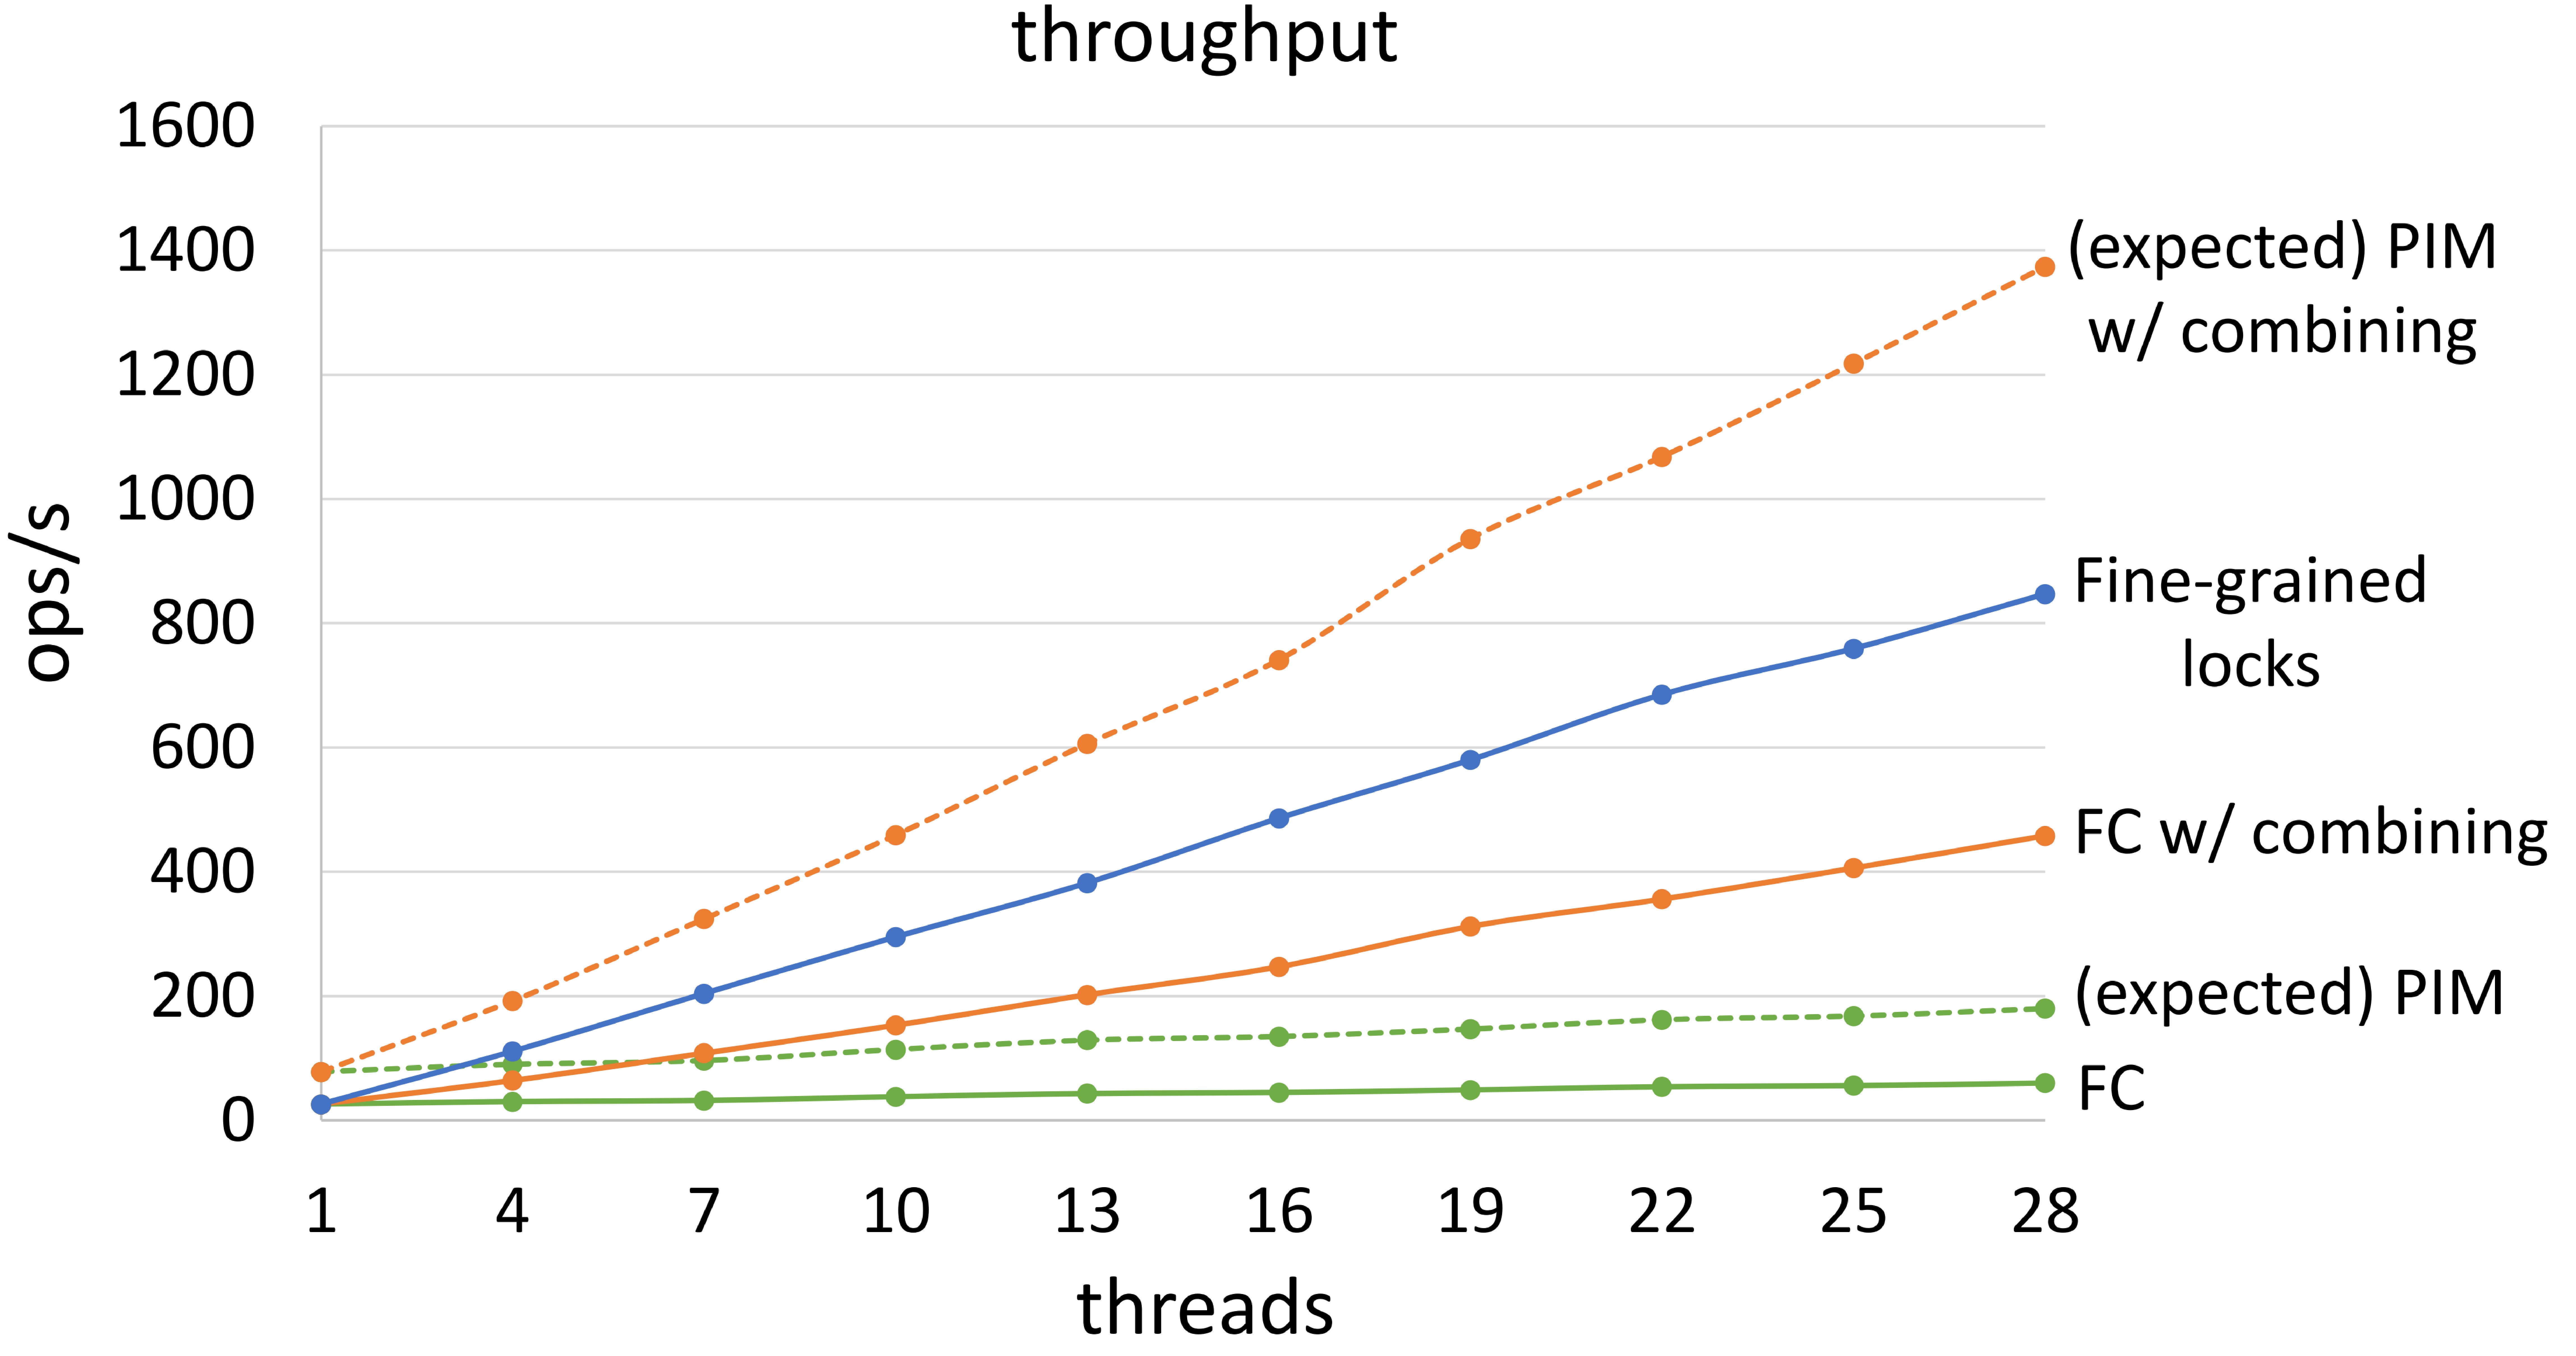
\includegraphics[width=.8\linewidth]{linkedlist_data.eps}
%$\hrulefill$
\caption{Experimental results of linked-lists}
\label{figure:linkedlist_data}
\end{figure}

\subsection{PIM-managed skip-list}
\label{section:skip_list}

\subsubsection{Base algorithm}
Like the naive PIM-managed linked-list,
the naive PIM-managed skip-list keeps the skip-list in a single vault and
CPUs send operation requests to the local PIM core which executes those operations.
As we will see, this algorithm is less efficient than some existing algorithms either.

Unfortunately, the combining optimization cannot be applied to skip-lists effectively.
The reason is that for any two nodes not close enough to each other in the skip-list,
the paths we traverse through to reach them don't largely overlap.

On the other hand, PIM memory usually consist of many vaults and PIM cores.
For instance, the first generation of Hybrid Memory Cube \cite{website:HMC} has 32 vaults.
Hence, a PIM-managed skip-list may achieve much better performance if
we can exploit the parallelism of multiple vaults and PIM cores.
Here we present our PIM-managed skip-list with \emph{partitioning optimization}:
A skip-list is divided into partitions of disjoint ranges of keys,
stored in different vaults, so that a CPU sends its operation request to
the PIM core of the vault to which the request belongs.

Figure \ref{figure:skiplist_structure} illustrates the structure of a PIM-managed skip-list.
Each partition of a skip-list starts with a \emph{sentinel node}
which is a node of the max height. For simplicity, assume the max height $H_{max}$ 
is predefined and each node in a skip-list has height between 1 and $H_{max}$.
The key range a partition covers is the between the key of its sentinel node and
the key of the sentinel node of the next partition.

CPUs also store a copy of each sentinel node in the normal DRAM of the PIM memory 
and the copy has an extra variable indicating the vault containing the sentinel node.
Since the number of nodes of the max height is very small with high probability, 
the copies of those sentinel nodes can almost for certain stay in cache
if CPUs access them frequently.

When a CPU wants to make an operation of some key to the skip-list,
it first compares the key with those of the sentinels, finds out the vault
the key belongs to, and then sends its operation request to
the PIM core of the vault.
Once the PIM core retrieves the request, it executes the operation in the local vault 
and finally sends the result back to the CPU.


\begin{figure}[ht!]
%$\hrulefill$
%\\
%\\
\centering
\includegraphics[width=.8\linewidth]{skiplist_structure.eps}
%$\hrulefill$
\caption{A PIM-managed FIFO queue with three partitions}
\label{figure:skiplist_structure}
\end{figure}

Now let us discuss how to implement our PIM-managed skip-list
when the key of each operation is an integer generated uniformly at random
from range $[0, n]$ and the PIM memory has $k$ vaults available.
In this case, we can initialize $k$ partitions starting with fake sentinel nodes
$0, 1/k, 2/k,..., (n-1)/k$, respectively.
We allocate one partition in a different vault and hence $k$ vaults cover
$k$ disjoint key ranges of size same.
The sentinel nodes will never be deleted.
If a new node to be added has the same key as a sentinel node,
we add it immediately after the sentinel node.

We compare the performance of our PIM-managed skip-list with partitions 
with the performance of a flat-combining skip-list \cite{Hendler10} with modifications
and a lock-free skip-list \cite{Herlihy08}, 
in a machine with $p$ CPUs and $k$ PIM vaults.
To simplify the comparison, we assume that all skip-lists have the same
initial structure (expect that skip-lists with partitions have extra sentinel nodes)
and all the operations are contains() operations
(or the number of $add()$ requests is almost the same as the number of $delete()$ 
so that the size of each skip-list nearly doesn't change).
Their approximate expected throughputs are as follows:

\begin{itemize}
\item Look-free skip-list:
	${p \over \beta\latcpu}$

\item Flat-combining skip-list without partitioning:
	${1 \over \beta\latcpu}$

\item PIM-managed skip-list without partitioning:
	${1 \over (\beta\latpim + \latmes)}$

\item Flat-combining skip-list with $k$ partitions:
    ${k \over \beta\latcpu}$

\item PIM-managed linked-list with $k$ partitions:
    ${k \over (\beta\latpim + \latmes)}$
\end{itemize}

where $\beta$ is the average number of nodes an operation has to go through
in order to find the location of its key in a skip-list
($\beta = \Theta(\log N)$, where $N$ is the size of the skip-list).
The flat-combining skip-list with $k$ partitions is one that has $k$ combiner locks,
each for a partition, so that CPUs compete for locks of partitions their operation
keys belong to.
Note that in the analytical results above, we ignored some overheads in the flat-combining
algorithms, such as maintaining combiner locks and combining arrays
(we will discuss combining arrays in more detail in Section \ref{section:contended}).
We also overestimated the performance of the lock-free skip-list by not counting the
CAS operations used in add() and delete() requests, as well as the cost of retries
caused by conflicts of updates.
Even so, our PIM-managed linked-list with partitioning optimization is
still expected to outperformance other algorithms when $k > p/3$.

Our experiments have revealed similar results, 
as presented in Figure \ref{figure:skiplist_data}.
We have implemented and run the flat-combining skip-list with different numbers of
partitions and compared them with the lock-free skip-list.
As the number of partitions increases, the performance of the flat-combining skip-list
gets better and better, implying the effectiveness of partitioning optimization.
Again we believe the performance of the flat-combining skip-list is a good indicator
to the performance of our PIM-managed skip-list.
Therefore, according to the analytical results we have shown, we can triple the throughput
of a flat-combining skip-list to get the expected performance of a PIM-managed skip-list.
As the figure illustrates, when the PIM-managed skip-list has $8$ or $16$ partitions,
it is expected to outperform the lock-free skip-list with up to 28 hardware threads.

\begin{figure}[ht!]
%$\hrulefill$
%\\
%\\
\centering

\includegraphics[width=.8\linewidth]{skiplist_data.eps}
%$\hrulefill$
\caption{Experimental results of skip-lists}
\label{figure:skiplist_data}
\end{figure}

\subsubsection{Rebalancing skip-list}
We have shown that our PIM-managed skip-list performs well with uniform distribution of requests. 
With non-uniform distribution of requests, we may need to periodically rebalance the skip-list 
in order to maintain good performance. 
Here we discuss how to migrate consecutive nodes from one vault to another without blocking requests.  

To move consecutive nodes from its local vault to another vault $v$, a PIM core $p$ 
can send messages of requests of adding those nodes to the local PIM core $q$ of $v$ as follows. 
First, $p$ sends a message notifying $q$ of the start of the node migration. 
Then $p$ sends messages of adding those nodes to $q$ one by one in an ascending order 
according to the keys of the nodes. 
After all those nodes have been migrated, $p$ sends notification messages to CPUs so that 
CPUs can update their copies of sentinel nodes accordingly.
Once $p$ receives acknowledgement messages from all CPUs, it notifies $q$ of the end of migration.
To keep the node migration protocol simple, we don't allow $q$ to move those nodes 
to another vault again until $v$ finishes its node migration. 

During this node migration, $p$ can periodically check its message buffer for requests from CPUs.
Assume that a request with key $k_1$ is sent to $p$ when $p$ is migrating nodes 
in a key range that $k_1$ is in.  
If $p$ is about to send a message to migrate a node with $k_2$ at the moment, where $k_1 \ge k_2$, 
$p$ serves the request itself. 
Otherwise $p$ forwards the request to $q$. 
In either case, $p$ can then continue its node migration without blocking concurrent requests. 
It is not hard to see the correctness of the node migration procedure 
with the presence of requests: a request will eventually reach the vault that 
currently contains nodes in the key range that the request is in.
If a request later arrives to $p$ which no longer holds the partition the request belongs to, 
$p$ can simply reply with a rejection to the sender CPU and 
the sender CPU will resend its request to the correct PIM core, 
because the CPU has already updated its sentinels and knows which PIM core it should contact. 

Using this node migration protocol, our FIFO queue can support two rebalancing schemes:
1) If a partition has too many nodes, the local PIM core can divide it into two smaller  
partitions (the first nodes of two smaller partitions are modified to have the max height 
in order to serve as sentinels) and migrate one of them to another PIM vault; 
2) If two consecutive partitions are both small, we can merge then by moving one to the vault 
containing the other. 
If rebalancing happens infrequently, its overhead is affordable. 

\subsubsection{Parallelism of memory accesses}
If the distribution of requests to the PIM-managed skip-list is very sharp, that is, 
a lot of requests hit a small range of keys, we may have to rebalance the skip-list too often, 
incurring significant performance overhead. 
However, if we don't rebalance the skip-list frequently, 
a large number of requests may be sent one PIM core, which becomes the performance bottleneck. 
On the other hand, even existing concurrent skip-list algorithms in which threads execute 
their operations by themselves in parallel cannot have good performance either, 
since concurrent updates (i.e., add() and delete()) within a small range conflict with one another. 
Thus, we believe a PIM-managed skip-list can achieve competitive throughput if each PIM core can 
execute multiple read-only requests (i.e., contains()) and at most one update request efficiently. 
We have assumed each PIM core can only deal with one request at a time, 
but in fact it has the potential to execute multiple requests in parallel.

Hsieh et al. \cite{hsieh2016accelerating} proposed how to design a PIM core that 
can make multiple memory accesses for multiple pointer-chasing based requests in parallel. 
The idea is that, after requiring a memory access for an operation request A, 
it can immediately retrieve another request B without waiting for the data of the memory access for A. 
The PIM core will later resume A once the data of the memory access is returned.  
In other words, the PIM core can hide its memory access latency by making multiple accesses in 
multiple requests in parallel. 
In theory, if the sum of the latency of doing the computation between two memory accesses 
for a pointer-chasing based request and the latency of switching from one request to another 
is only $1/k$ of the latency of a memory access by the PIM core, 
the PIM core can essentially execute $k$ requests in parallel without 
delaying the pointer-chasing procedure of each request (see \cite{} (TBD) for more detail). 
Those requests can therefore be thought of as requests executed in parallel
by different hardware threads of the PIM core. 

Now we explain in detail how each kind of requests to a PIM-managed skip-list is executed. 
For a contains($x$) request of key $x$, a PIM core simply does the search procedure for key $x$
as in a normal sequential skip-list algorithm. 
For an add($x$) request, The PIM core also does the same search procedure first. 
If a node of key $x$ already exists in the skip-list, the execution is completed.
Otherwise, the search procedure must has collected the predecessor and successor nodes 
between which a new node of key $x$ will be inserted 
(see \cite{Herlihy08} for more details, where the search procedure is denoted as the find function). 
The new node of random height is then generated and inserted \textbf{from the bottom layer up}: at each layer, 
the PIM core first sets the ``next node" pointer of the new node to point to its successor at the layer 
and then sets the ``next node" pointer of its predecessor at the layer to point to the new node. 
Similarly, for a delete($x$) request, the PIM core first does the search for key $x$. 
If a node with key $x$ is in the skip-list, the PIM core removes it \textbf{from the top layer down}: 
at each layer, the PIM core sets the ``next node" pointer of the node's predecessor to point to its successor.
To free the memory space of the node, the PIM core can later physically deleted it, either in a quiescent 
state, or after the PIM core have completed another $k$ requests, since there are at almost $k$ contains() 
requests executed concurrently with the delete($x$) request and requests after that will never reach the node. 

Now we prove that this PIM-managed skip-list is linearizable. 

\proof
What we need to prove is that each partition of the PIM-managed skip-list, 
which is essentially a skip-list within a smaller range of keys in a single PIM vault, 
is linearizable when there are at most one update request and multiple contains() executed concurrently.   

We start with the linearization points of requests. 
For a contains($x$) request that finds a node with key $x$ in the skip-list at some layer, 
its linearization point is the moment the PIM core reads the predecessor of the node at that layer. 
For a contains($x$) request that doesn't find a node with key $x$, its linearization point is the moment 
the PIM core reads the predecessor of the first node with key greater than $x$ at the bottom layer 
(i.e., the node at the bottom layer in the ``predecessor array" return by the find($x$) function \cite{Herlihy08}). 
For an unsuccessful update to $x$, that is, a delete($x$) that doesn't find an existing node with key $x$ 
or an add($x$) that finds an existing node with key $x$), 
its execution is in fact the same as that of a contains($x$) and so does its linearization point. 
For a successful add($x$) (which doesn't find an existing node with key $x$ and needs to insert a new node), 
its linearization point is the moment the PIM core modifies the ``next node" pointer of the predecessor 
of the new node at the bottom layer to point to the new node 
(that is, the step of inserting the new node at the bottom layer).  
For a successful delete($x$) (which finds an existing node with key $x$), its linearization point is 
the moment the PIM core modifies the ``next node" pointer of the predecessor of the node to point to 
the successor of the node at the bottom level (that is, the step of removing the node at the bottom layer). 

Since update requests are executed sequentially and contains() requests are read-only, 
it is obvious that the results (i.e., responses) of update requests are consistent 
with the sequential history defined by the linearization points we just described. 
To see that a contains($x$) request is also correctly linearized, we first consider the case where 
the last successful update to $x$ linearized before contains($x$) is a successful add($x$) and 
the first successful update to $x$ linearized after contains($x$) is a successful delete($x$). 
We can prove that contains($x$) must find a node with key $x$, consistent with the sequential history. 
To prove it by contradiction, we assume contains($x$) doesn't find such a node and hence is linearized 
at the moment it reads the predecessor of the first node with key greater than $x$ at the bottom layer. 
However, since the last successful update to $x$ linearized before contains($x$) is a successful add($x$), 
a node with key $x$ must have been inserted between the node contains($x$) is about to read and the first 
node with key greater than $x$ at the first layer, according to the way we linearize a successful add($x$). 
Therefore the node contains($x$) is about to read cannot pointer to a node with key greater than $x$, 
a contradiction, and hence contains($x$) must find a node with key $x$. 
By very similar proofs that are omitted here, we can show that a contains($x$) is also correctly linearized 
when the last successful update to $x$ linearized before contains($x$) is a successful delete($x$), or
the first successful update to $x$ linearized after contains($x$) is a successful add($x$). 
This completes the proof. 
\qed


\section{Contended Data Structure}
\label{section:contended}
In a contended concurrent data structure, operations have to compete for
accessing some contended spots and
such contention is the performance bottleneck of the data structure.
Examples are stack and different kinds of queues.

The contended data structure we focus on is FIFO queue, where concurrent enqueue
and dequeue operations need to compete for the head and tail of the queue, respectively.
In existing concurrent FIFO queue algorithms, enqueue and dequeue usually
make CAS or F\&A to compete for the head and tail pointers of the queue.

A contended data structure like a FIFO queue usually has good cache locality
and doesn't need long pointer chasing to complete an operation.
In a concurrent FIFO queue, for instance, the head and tail pointer can stay in
cache if they are accessed frequently by CPUs directly, and each enqueue or dequeue
operation only needs to access and update one or two pointers before completing its operation.
One may think the PIM memory is therefore not a suitable platform for such a data structure,
since now we cannot make good use of the fast memory access of PIM cores, but also
lose the performance boosting provided by CPUs' cache.
However, we are going to show a somewhat counterintuitive result that we can still design
a PIM-managed FIFO queue that outperforms other existing algorithms.

\subsection{PIM-managed FIFO queue}
The structure of our PIM-managed FIFO queue is shown in Figure \ref{figure:queue_structure}.
A queue consists of a sequence of segments, each containing consecutive nodes of the queue.
A segment is allocated in a PIM vault, with a head node and a tail node pointing to the first 
and the last nodes of the segment, respectively.
A vault can contain multiple (mostly likely non-consecutive) segments. 
There are two special segments---the \emph{enqueue segment} and the \emph{dequeue segment}.
To enqueue a node, a CPU sends an enqueue request to the PIM core of the vault
that contains the enqueue segment.
The PIM core will then insert the node to the head of the segment.
Similarly, to dequeue a node, a CPU sends a dequeue request to the PIM core of the vault
holding the dequeue segment. 
The PIM core will pop out the node at the tail of the dequeue segment and 
send the node back to the CPU.

Initially the queue consists of an empty segment which acts as both the enqueue segment and 
the dequeue segment. 
When the length of enqueue segment exceeds some threshold, the PIM core maintaining it
notifies another PIM core to create a new segment as the new enqueue segment.\footnote{
When and how to create a new segment can be decided in other ways.
For example, CPUs, instead of the PIM core holding the enqueue segment, 
can decide when to create the new segment and which vault to hold the new segment, 
based on more complex criteria 
(e.g., if a PIM core is currently holding the dequeue segment, it will not be chosen for 
the new segment so as to avoid the situation where it deals with both enqueue and dequeue requests).
To simplify the description of our algorithm, we omit those variants.}
When the dequeue segment becomes empty and the queue has one than one segment at the moment, 
the dequeue segment is deleted and the segment that were created first 
among all the remaining segments is designated as the new dequeue segment. 
(It is not hard to see that the new dequeue segment were created when the old dequeue segment 
acted as the enqueue segment and exceeded the length threshold.)
When the enqueue segment is different from the dequeue segment, 
enqueue and dequeue operations can be executed by two different PIM cores 
in parallel, which doubles the throughput compared to a straightforward queue implementation 
maintained in a single vault.  

\begin{figure}[ht!]
%$\hrulefill$
%\\
%\\
\centering
\includegraphics[width=.8\linewidth]{queue_structure.eps}
%$\hrulefill$
\caption{A PIM-managed FIFO queue with three segments}
\label{figure:queue_structure}
\end{figure}



\begin{figure}
\begin{algorithm}[H]
\SetKwInOut{Input}{input}\SetKwInOut{Output}{output}
\Input{\textbf{enq(cid, \textit{u})}}
\Begin
{
	\eIf{enqSeg == null}
    {
        send message(cid, false)\;
    }
    {
        \eIf{enqSeg.head $\ne$ null}
        {
            enqSeg.head.next = $u$\;
            enqSeg.head = $u$\;
        }
        {
            enqSeg.head = $u$\;
            enqSeg.tail = $u$\;
        }

        enqSeg.count = enqSeg.count + 1\;
        send message(cid, true)\;

        \If{enqSeg.count $>$ threshold}
        {
            cid$'$ = the CID of the PIM core chosen to maintain the new segment\;
            send message(cid$'$, newEnqSeg())\;
            enqSeg.nextSegCid = cid$'$\;
            enqSeg = null;
        }
    }
}
\end{algorithm}
\caption{PIM core's execution upon receiving an enqueue request.}
\label{figure:enq}
\end{figure}

\begin{figure}
\begin{algorithm}[H]
\SetKwInOut{Input}{input}\SetKwInOut{Output}{output}
\Input{\textbf{deq(cid)}}
\Begin
{
    \eIf{deqSeg == null}
    {
        send message(cid, false)\;
    }
    {
        \eIf {deqSeg.tail $\ne$ null}
        {
			send message(cid, deqSeg.tail)\;
            deqSeg.tail = deqSeg.tail.next\;   
        }
        {
			\eIf {deqSeg == enqSeg}
			{
				send message(cid, null)\;
			}
            {
                send message(deqSeg.nextSegCid, newDeqSeg())\;
                deqSeg = null\;
                send message(cid, false)\;
            }            
        }
    }
}
\end{algorithm}
\caption{PIM core's execution upon receiving a dequeue request.}
\label{figure:deq}
\end{figure}

\begin{figure}
\begin{algorithm}[H]
\SetKwInOut{Input}{input}\SetKwInOut{Output}{output}
\Input{\textbf{newEnqSeg()}}
\Begin
{
    enqSeg = new Segment() \;
    segQueue.enq(engSeg) \;
    notify CPUs of the new enqueue segment\;
}
\end{algorithm}

\begin{algorithm}[H]
\SetKwInOut{Input}{input}\SetKwInOut{Output}{output}
\Input{\textbf{newDeqSeg()}}
\Begin
{
    deqSeg = segQueue.deq() \;
    notify CPUs of the new dequeue segment\;
}
\end{algorithm}	
\caption{Functions to create and retrieve new segments.}
\label{figure:newSegment}
\end{figure}

The pseudocode of our FIFO queue algorithm is presented in 
Figures \ref{figure:enq}-\ref{figure:newSegment}. 
Each PIM core has local variables enqSeg and deqSeg that are references to segments.
When enqSeg (respectively deqSeq) is not null, it is a reference to the enqueue 
(respectively dequeue) segment and indicates that the PIM core is currently holding 
the enqueue (respectively dequeue) segment.
Each PIM core also maintains a local queue segQueue for storing local segments.
CPUs and PIM cores communicate via message(cid, content) calls, where cid is the unique core ID (CID) 
of the receiver and the content is either a request or a response to a request.

Once a PIM core receives an enqueue request enq(cid, $u$) of node $u$ from a CPU whose CID is cid,
it first checks if it is holding the enqueue segment (line 2 in Figure \ref{figure:enq}).
If so, the PIM core enqueues $u$ (lines 5-13), and otherwise sends back a message
informing the CPU that the request is rejected (line 3) so that
the CPU can resend its request to the right PIM core holding the enqueue segment
(we will explain later how the CPU can find the right PIM core).
After enqueuing $u$, the PIM core may find the enqueue segment is longer than the threshold (line 14).
If so, it chooses the PIM core of another vault for creating and maintaining a new enqueue segment 
and sends a message with a newEnqSeg() request.
Finally it sets its enqSeq to null indicating it no longer deals with enqueue operations.
Note that the CID cid' of the PIM core chosen for creating the new segment is recorded in 
enqSeg.nextSegCid for future use in dequeue requests.
As Figure \ref{figure:newSegment} shows,
The PIM core receiving this newEnqSeg() request creates a new enqueue segment and enqueues 
the segment into segQueue (line 3). 
Finally it notifies CPUs of the new enqueue segment (we will get to it in more detail later).

Similarly, when a PIM core receives a dequeue request deq(cid) from a CPU with CID cid,
it first checks if it still holds the dequeue segment (line 2 of Figure \ref{figure:deq}).
If so, the PIM core dequeues a node and sends it back to the CPU (lines 5-7).
Otherwise, the PIM core informs the CPU that this request has failed (line 3) and
the CPU will have to resend its request to the right PIM core.
If the dequeue segment is empty (line 8) and the dequeue segment is not the same as 
the enqueue segment (line 11), which indicates that the FIFO queue is not empty 
and there exists another segment, the PIM core sends a message with a newDeqSeg() request 
to the PIM core with CID deqSeg.nextSegCid. 
(We know that this PIM core must hold the next segment, 
according to how we create new segments in enqueue operations, 
as shown at lines 15-17 in Figure \ref{figure:enq}.) 
Upon receiving the newDeqSeg() request, as illustrated in Figure \ref{figure:newSegment}, 
the PIM core retrieves the oldest segment it has created and makes it the new dequeue segment.    Finally the PIM core notifies CPU that it is holding the new dequeue segment now.

Now we explain how CPUs and PIM cores coordinate to make sure that CPUs can find the right enqueue 
and dequeue segments, when their previous attempts have failed due to changes of those segments. 
We will only discuss how to deal with enqueue segments here, 
since the same methods can be applied to dequeue segments. 
A straightforward way to inform CPUs is to have the owner PIM core of the new enqueue segment 
send notification messages to them (line 4 of newEngSeg() in Figure \ref{figure:newSegment}) 
and wait until they all send back acknowledgement messages. 
However, if there is a slow CPU that doesn't reply in time, 
the PIM core has to wait for it and therefore other CPUs cannot have their requests executed. 
A more efficient, non-blocking method is to have the PIM core start working for new requests 
immediately after it has sent off those notifications. 
CPUs don't have to reply to those notifications in this case, but they need to send messages 
to (all) PIM cores to ask whether they are in charge of the enqueue segment, 
if their requests have failed.
In either case, the correctness of the algorithm is guaranteed:  
at any time, there is only one enqueue segment and only one dequeue segment, 
only requests sent to them will be executed. 
  
We would like to mention that the PIM-managed FIFO can be further optimized. 
For example, the PIM core holding the enqueue segment can combine multiple pending enqueue requests 
and store the nodes to be enqueued in an array as a ``fat" node of the queue, 
so as to reduce memory accesses. 
This optimization is also used in the flat-combining FIFO queue \cite{Hendler10}. 
Even without this optimization, our algorithm still performs well, as we will show next. 

\subsection{Performance analysis}
We will compare the performance of three concurrent FIFO algorithms---our PIM-manged FIFO queue, 
a flat-combining FIFO queue and the F\&A-based FIFO queue \cite{Morrison13}. 
The F\&A-based FIFO queue is the most efficient concurrent FIFO queue we are aware of, 
where threads make F\&A operations on two shared variables, 
one for enqueues and the other for dequeues, to compete for the slots in the FIFO queue to 
enqueue and dequeue nodes (see \cite{Morrison13} for more details). 
The flat-combing FIFO queue we consider is based on the one proposed by \cite{Hendler10}, 
after our modifications, so that threads compete for two ``combiner locks", 
one for enqueues and the other for dequeues, 
and we simplify it by assuming the queue is always non-empty so that it doesn't have to deal with 
the synchronization issue between an enqueue and a dequeue when the queue is empty. 

We start with the analysis of the algorithms when a queue is long enough such that the PIM-managed 
FIFO queue has more than one segment and 
therefore enqueue and dequeue requests can are executed separately. 
Since creating and changing enqueue and dequeue segments happens very infrequently, its overhead is negligible and assume it never happens in order to simplify our performance analysis.
(If the threshold of segment length at line 14 in Figure \ref{figure:enq} is some large integer $n$, 
then, in the worst case, changing enqueue segment can happen only once every $n$ enqueues and 
changing dequeue segment can happen only once every $n$ dequeues. 
Also, the cost of do so is only the latency of sending one message and a few steps of local computation.)

Since enqueues and dequeues are isolated, we focus on dequeues here,
and the analysis of enqueues is almost identical. 
Assume there are $p$ concurrent dequeue requests by $p$ CPUs. 
Since each CPU needs to make a F\&A operation on a shared variable in the F\&A-based algorithm and 
F\&A operations on a shared variable are essentially serialized, 
the execution time of $p$ requests in the algorithm is at least $p\latato$. 
Similarly, if we assume a CPU makes a request immediately after its previous request is completed, 
we can prove that the throughput of the algorithm is at most ${1 \over \latato}$.

In the flat-combining FIFO queue, the flat combiner has to go through the combining array to 
retrieve pending requests and later write results back to the combining array. 
Since other CUPs with pending requests spin on this shared combining array, 
each access by the flat combiner to a slot of the combining array incurs at least a last-level cache access. 
Therefore, the execution time of $p$ requests in the algorithm is at least $2p\latllc$ and 
the throughput of the algorithm is at most ${1 \over 2\latllc}$.

Note that we made quite optimistic analysis for the F\&A-based and flat-combining algorithms 
by counting only the costs in part of their executions and ignoring their performance degrading under contention. 
For example, under heavy contention, the F\&A-based algorithm may suffer significant performance degradation 
because contended atomic operations, such as F\&A and CAS, usually perform much worse in practice.  
Also, the latency of accessing and modifying nodes by a flat combiner is ignored here. 
For dequeue requests, this latency can be very high: since nodes to be dequeued in a long queue is unlikely to 
be cached, a flat combiner has to make a sequence of memory accesses to dequeue them one by one.  

\begin{figure}[ht!]
%$\hrulefill$
%\\
%\\
\centering
\subfigure[]{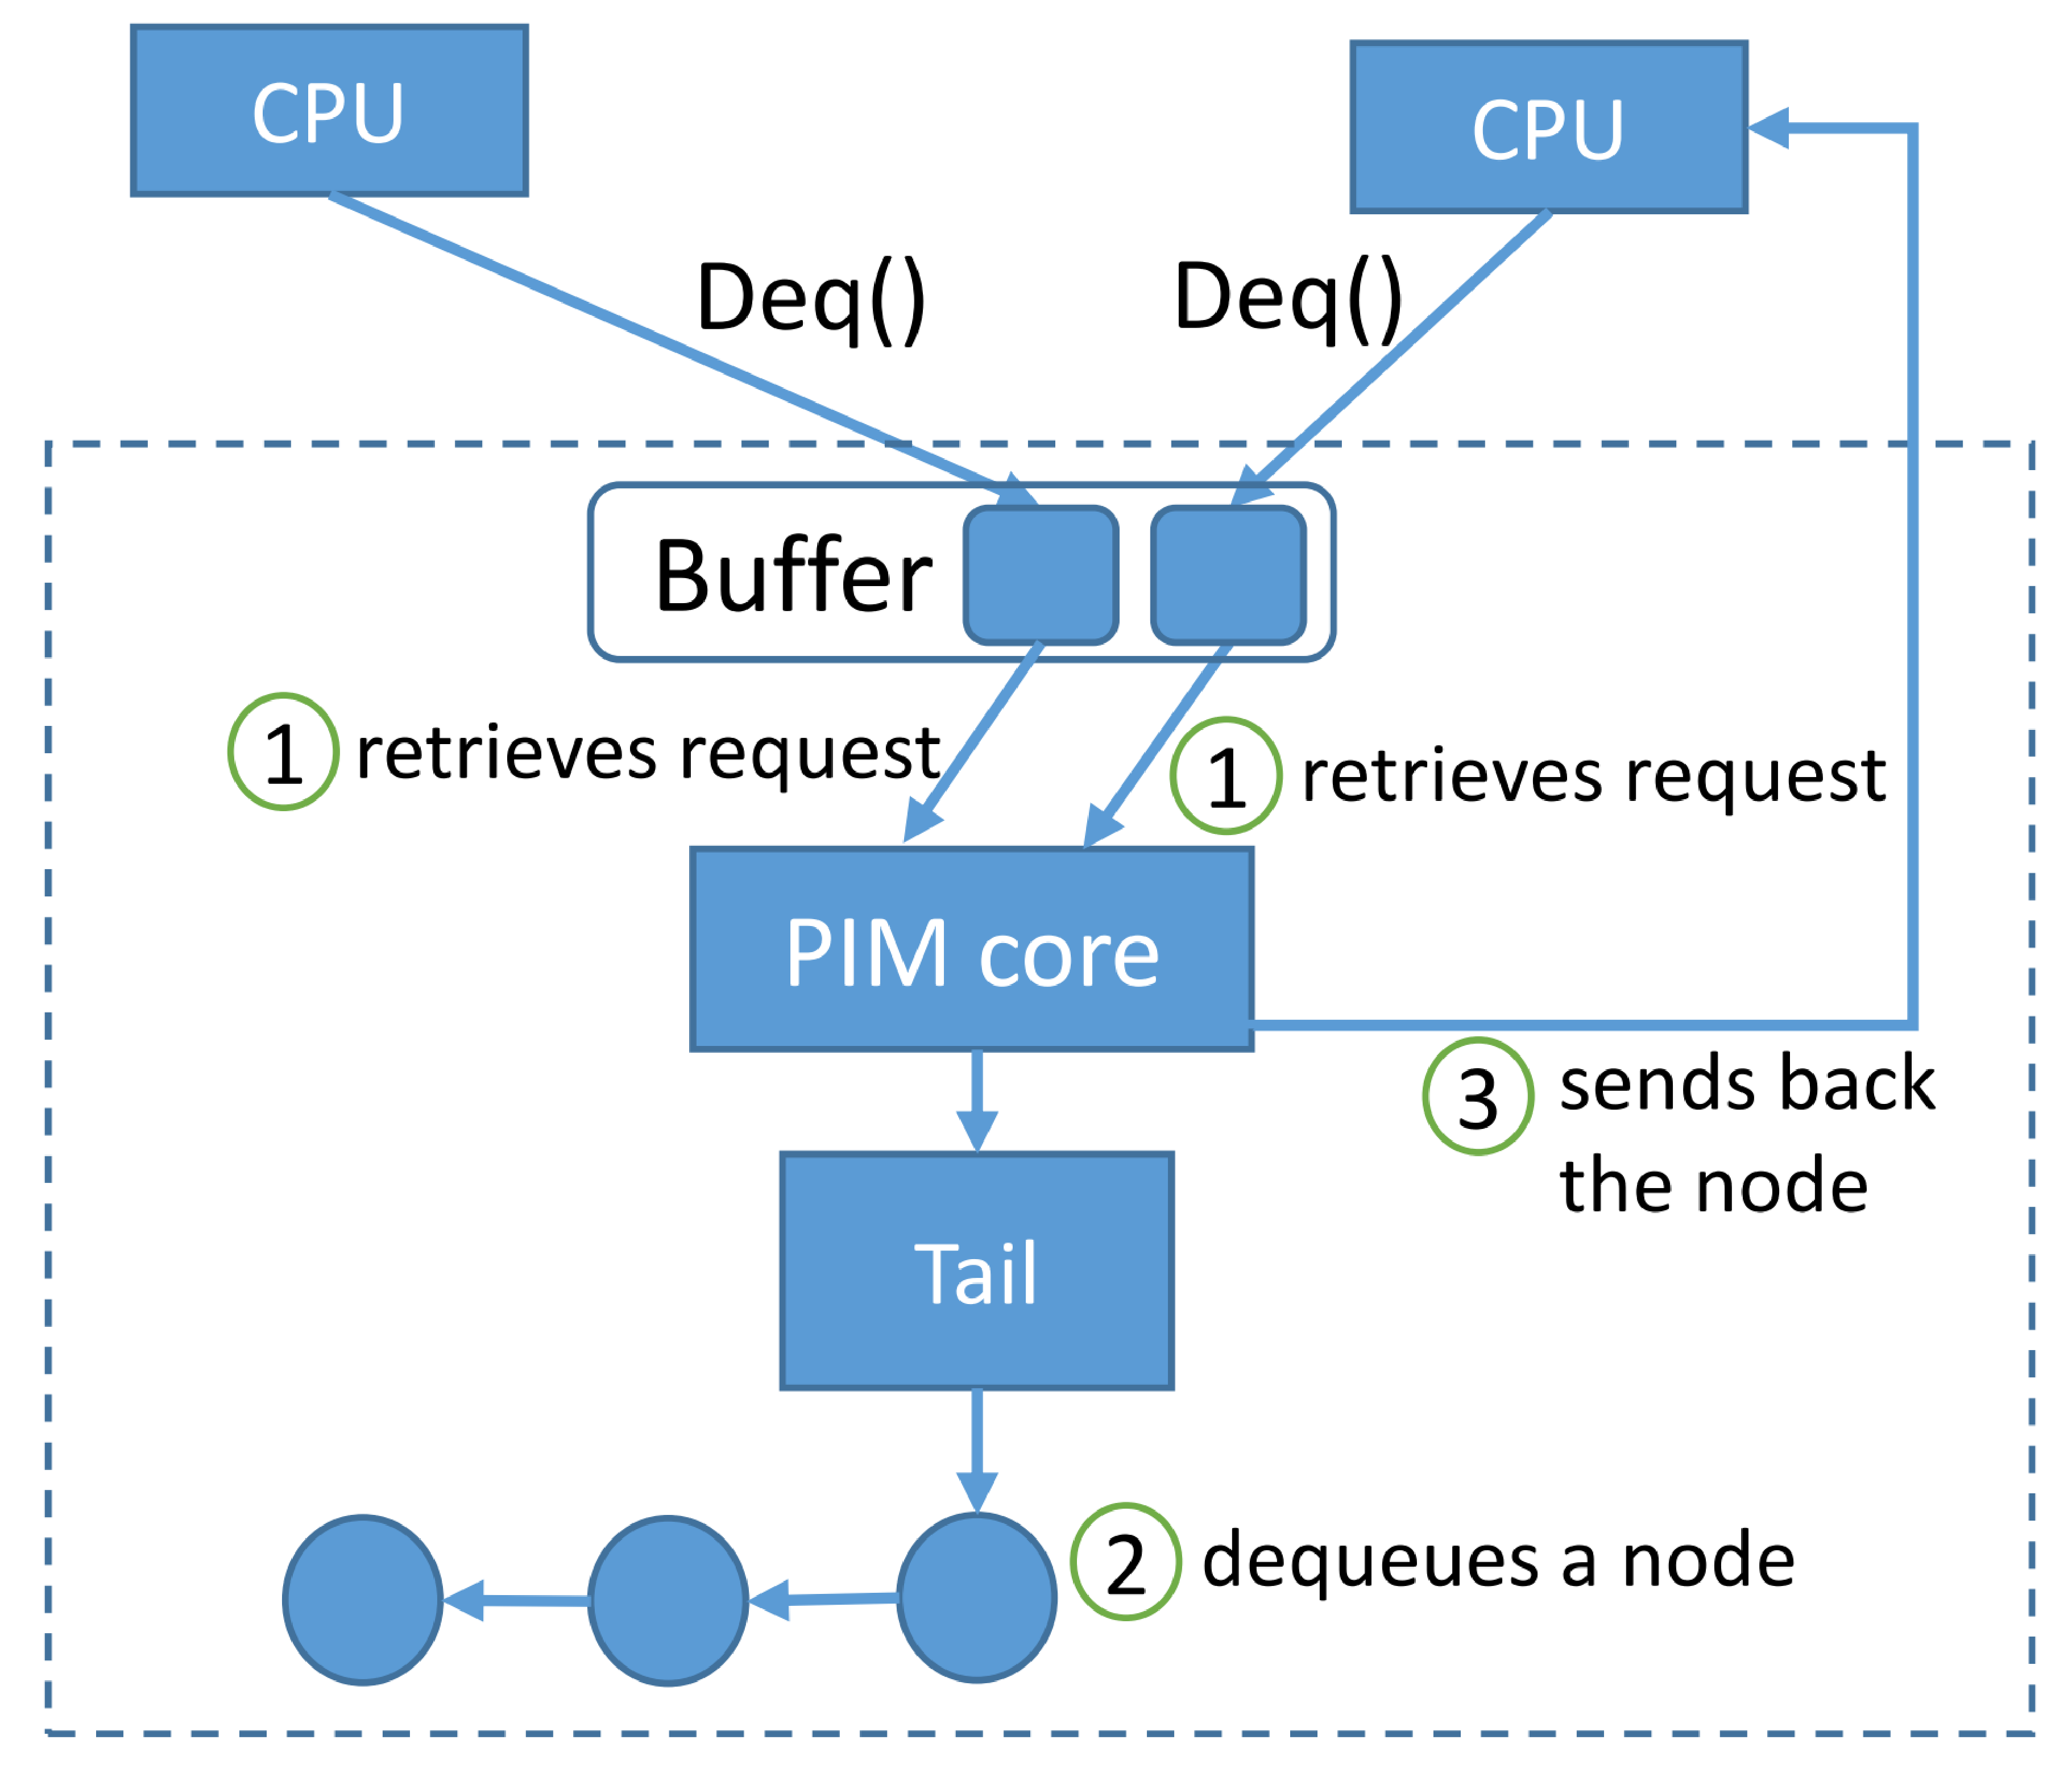
\includegraphics[width=.45\linewidth]{queue_pipeline.eps}}
\subfigure[]{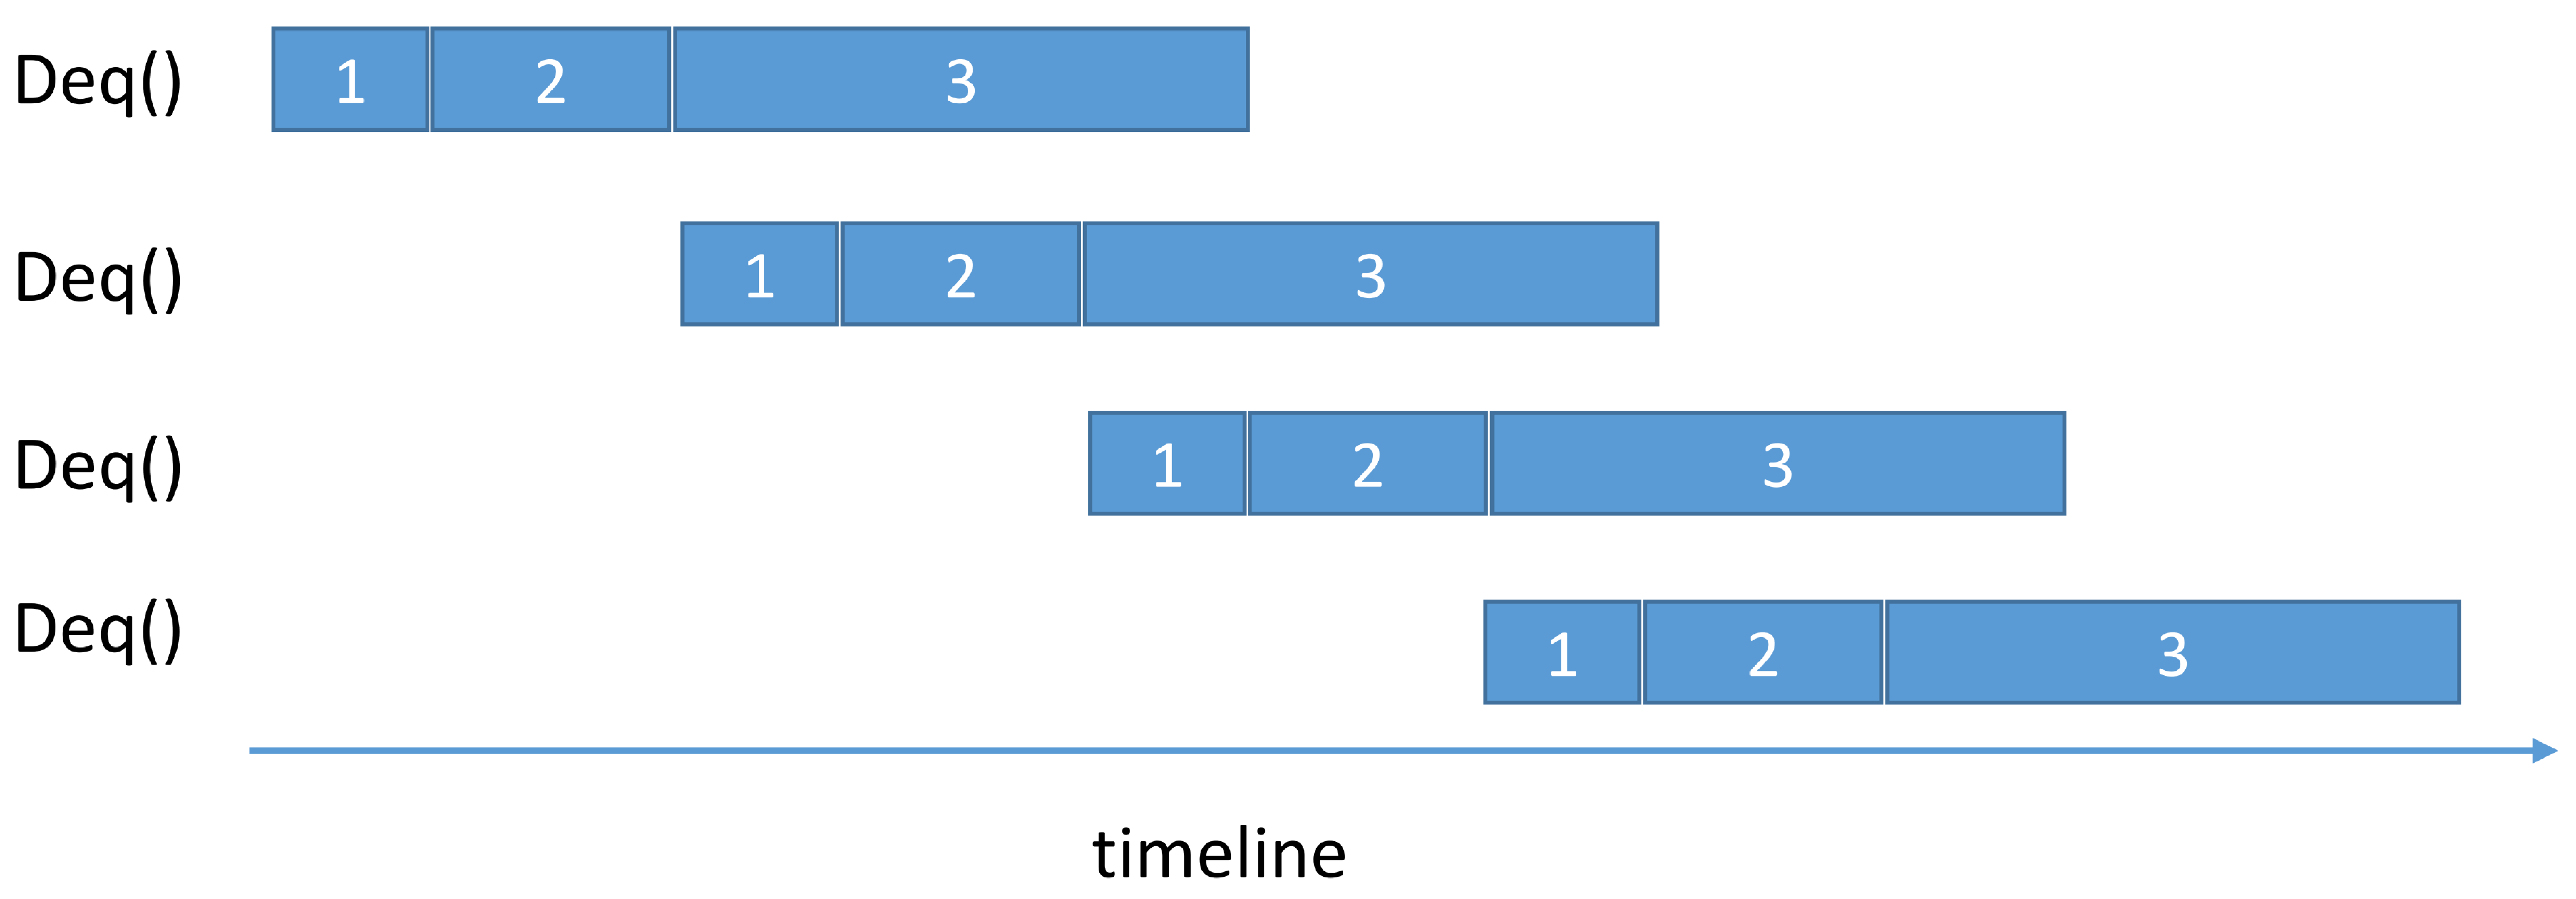
\includegraphics[width=.45\linewidth]{queue_pipeline_timeline.eps}}

%$\hrulefill$
\caption{(a) illustrates the pipelining optimization, where a PIM core can start executing a new 
deq() (i.e., step 1 of deq() for the CPU on the left), without waiting for the dequeued node of the previous deq() 
to get back to a CPU (step 3 of the deq() for the CPU on the right). 
(b) shows the timeline of pipelining the three steps of four deq() requests.}
\label{figure:queue_pipeline}
\end{figure}

The performance of our PIM-managed FIFO queue seems poor at first sight: although a PIM core can update 
the queue efficiently, it takes a lot of time for the PIM core to send results back to CPUs one by one. 
However, its performance can be much improved, if we have the PIM core \textit{pipeline} 
the executions of requests as follows. 
Suppose $p$ CPUs send $p$ dequeue requests concurrently to the PIM core, which takes time $\latmes$. 
The PIM core fist retrieves a request from its message buffer (step 1 in the figure), 
dequeues a node (step 2), and sends the node back to a CPU (step 3). 
Note that, after the PIM core sends off the message containing the node, it can immediately retrieve the next 
request in its buffer, without waiting for the message to arrive at its receiver 
(see Figure \ref{figure:queue_pipeline}). 
Therefore, the PIM core can pipeline requests by overlapping the latency of message transfer (step 3) 
and the latency of memory accesses and local computations (steps 1 and 2) in multiple request. 
Note that, during the execution of a dequeue, the PIM core only needs one memory access to read the node 
to be dequeued, and two L1 cache accesses to read and modify the tail node 
when the tail node is accessed frequently and hence cached by the PIM core.  
It is easy to show that the execution time of $p$ requests is only $\latmes + p(\latpim + \epsilon) + \latmes$, 
where $\epsilon$ is the total latency of two L1 cache accesses, local computation and sending off the message, 
which is negligible in our performance model. 
If we assume a CPU makes a request immediately after its previous request is completed, 
we can prove that the throughput of the PIM-managed FIFO queue is 
$${1 - 2\latmes \over \latpim + \epsilon} \approx {1 - 2\latmes \over \latpim} 
\approx {1 \over \latpim}$$

Hence, the throughput of the PIM-managed FIFO queue is expected at least twice the throughput of each of 
the other two algorithms in our performance model assuming $\latato = 3\latllc = 3\latpim$, 
when the PIM-managed FIFO queue has more than one segment. 

When a queue is short, the PIM-managed FIFO queue may always have only one segment 
which deals with both enqueue and dequeue requests. 
In this case, the throughput of the PIM-managed FIFO queue is only half of that in the case when 
the queue consists of more than one segment, but still at least as good as the other two algorithms. 


\bibliographystyle{abbrv}
\bibliography{refs_pim}



\end{document}  